\chapter{Track Simulation}
	In order to develop and test the~reconstruction algorithm, electron and positron tracks are simulated inside our detector with different initial parameters. Three approaches are used to simulate tracks for different purposes.
	
	The~\textbf{Microscopic Simulation} uses the~Garfield++ toolkit~\cite{Garfield++}. Within this toolkit, the~\ac{HEED} program~\cite{HEED} is used to simulate the~primary particle and the~class \textit{AvalancheMicroscopic} to simulate the~drift of secondary electrons created by ionization in the~gas. This is the~most precise and time-consuming simulation used; our current goal is to be able to successfully reconstruct its results and determine our best-case energy resolution.
	
	The~\textbf{Runge-Kutta Simulation} uses the~4th order Runge-Kutta numerical integration (\textcolor{red}{add citation for Runge-Kutta}) to simulate the~trajectory of the~primary particle in the~electromagnetic field inside the~detector. It is relatively fast since it does not simulate the~secondary particles. It is used as part of our reconstruction algorithm and for testing some parts of the~reconstruction.
	
	The~\textbf{Fast Simulation with Ionization Electron Map} is planned for the~future. It will use the~\ac{HEED} program~\cite{HEED} to simulate the~primary particle and the~Ionization Electron Map (see Section~\ref{sec:map}) to simulate the~drift of secondary electrons. It should be significantly faster than the~Microscopic Simulation but offer comparable precision since it will rely on an already simulated drift map.
	
	All of these simulations require the~knowledge of the~electromagnetic field inside the~detector. A~uniform electric field of 400~V$\cdot$cm$^{-1}$ is assumed. The~magnetic field was simulated in Maxwell (\textcolor{red}{add citation? details? own subsection with figures? more details in Section~\ref{sec:IEAP}?}).
	
	\textcolor{red}{Could also mention mention Monte Carlo (requires gas file generation) and Runge Kutta simulation implemented in Garfield, why we don't use them.}
	\textcolor{red}{Single track in positive x direction or initial parameter randomization. Importance of gas composition, used gas compositions.}
	
	\section{Microscopic Simulation}
	\label{sec:microsim}
		The~microscopic simulation, the~most detailed simulation used in this work, is performed using the~Garfield++ toolkit~\cite{Garfield++} for this purpose. 
		
		The~electron transport properties are simulated using the~program Magboltz~(\textcolor{red}{Add citation.}). Two different gas mixtures were used: 90\%~Ar~+~10\%~CO$_2$ and 70\%~Ar~+~30\%~CO$_2$. The~second mixture will be used in our detector. The~temperature is set to 20~$^\circ$C, the~pressure is atmospheric.
		
		The~primary track is simulated using the~program~\ac{HEED}~\cite{HEED}, which is an implementation of the~photo-absorption ionization model. This program provides the~parameters of ionizing collisions. \ac{HEED} can also be used to simulate the~transport of delta electrons; we do not account for these in the~current simulation but plan to include them in the~future. The~photons created in the~atomic relaxation cascade (\textcolor{red}{fluorescence reabsorption, ?}) are also not simulated.
		
		Finally, we use the~microscopic tracking provided by the~class \textit{AvalancheMicroscopic} to simulate the~drift of the~ionization electrons. Each electron is followed from collision to collision using the~equation of motion and the~collision rates calculated by Magboltz.
		
		\textcolor{red}{First simulated track in the~$z$ direction. Figures.}
		
		\begin{figure}[H]
			\centering
			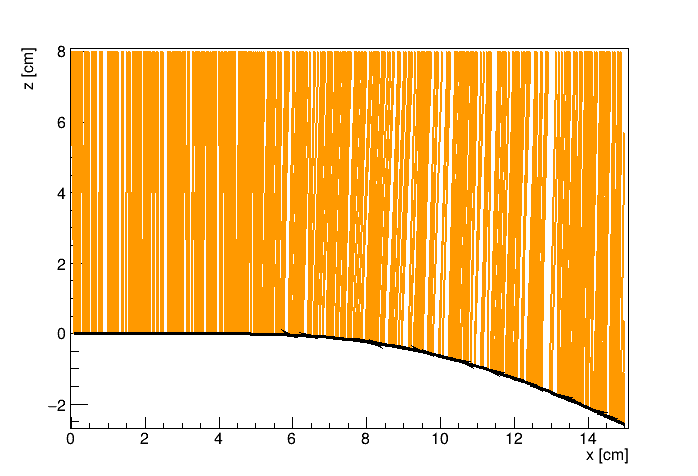
\includegraphics[width=0.3\textwidth]{7030_xz.png}
			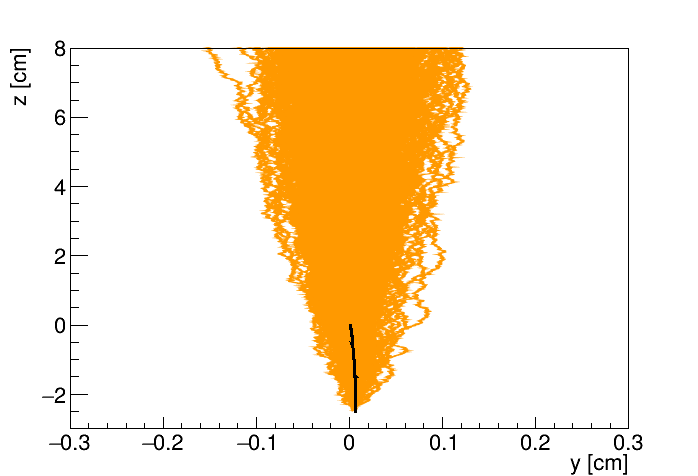
\includegraphics[width=0.3\textwidth]{7030_yz.png}
			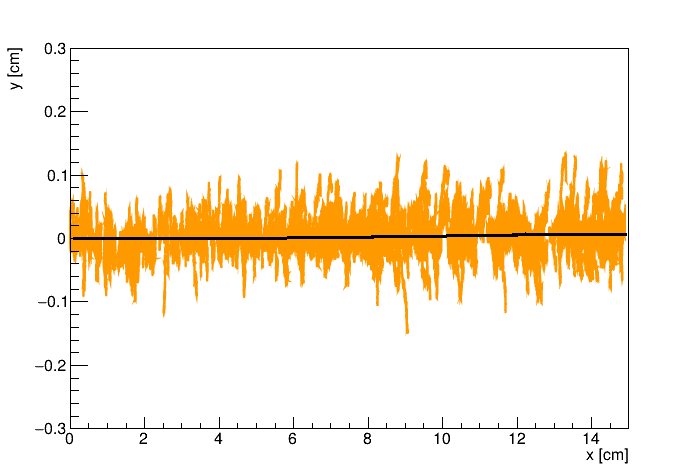
\includegraphics[width=0.3\textwidth]{7030_xy.png}
			\caption{Example of a~simulated electron track in 70~\%~argon and 30~\%~CO$_2$ atmosphere (on the~left). \textcolor{red}{Swap for better images, better zoom. Explain drift lines, primary particle.}}
			\label{fig:7030sim}
		\end{figure}
		
		\begin{figure}[H]
			\centering
			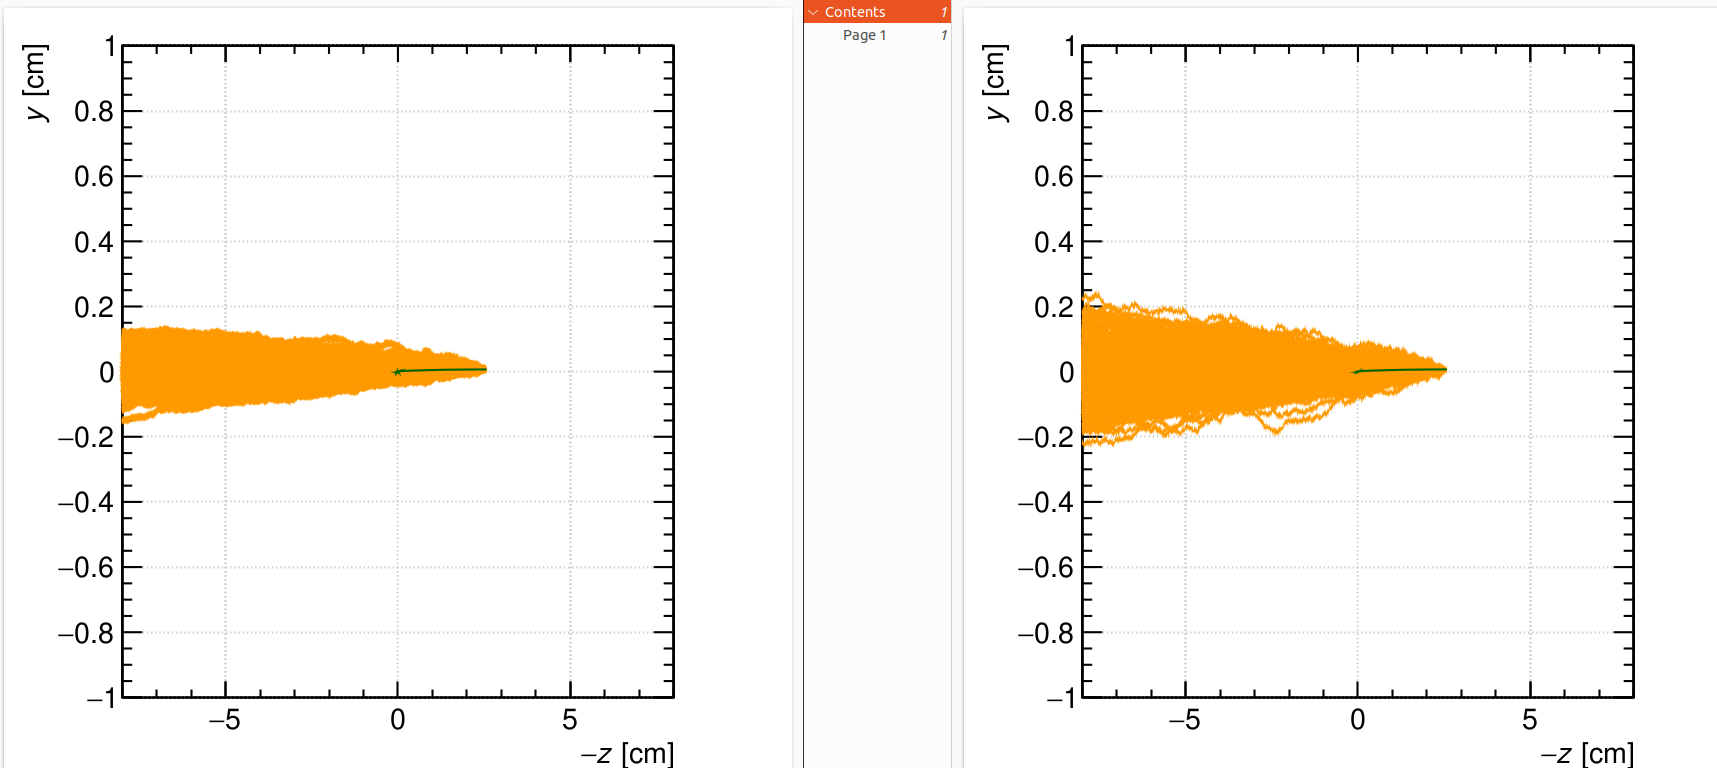
\includegraphics[width=0.9\textwidth]{diff_comp.png}
			\caption{Comparison of diffusion in a~simulated electron track in 70~\%~argon, 30~\%~CO$_2$ atmosphere and in 90~\%~argon, 10~\%~CO$_2$ atmosphere (on the~right). \textcolor{red}{Swap for better image, better zoom. Or put the~same pictures for both comparisons in one subfigure, etc. Describe better.}}
			\label{fig:diffcomp}
		\end{figure}
	
	\section{Runge-Kutta Simulation}
	\label{sec:rks}
		\textcolor{red}{Trajectory simulation with 4th order Runge-Kutta. Relativistic equation that is numerically integrated by the~algorithm.}
	
	\section{Future?: Fast Simulation with the~Ionization Electron Map}
		\textcolor{red}{Primary track simulated in HEED. Readout parameters by interpolating the~map. Diffusion from the~map for randomization.}